\chapter{Wie ich Newton Polygone zeichne}
\lstdefinestyle{myLatex} { 
  %language=[LaTeX]TeX
  language=LaTeX
  , texcsstyle=*\bf\color{blue} 
  , basicstyle=\ttfamily
  , numbers=none
  , breaklines=true
  , commentstyle=\color{red}
  %, otherkeywords={$, \{, \}, \[, \]} 
  %, frame=lines 
  , xleftmargin=30pt          % linker Abstand vom Rand (framesep+framrule)
  , tabsize=2
  %, caption=LaTeX example
}

Ich benutze tikz
\begin{lstlisting}[style=myLatex]
\usepackage{tikz}
\usetikzlibrary{matrix,arrows,decorations.pathmorphing}
\end{lstlisting}
und ein eigenes Kommando
\begin{lstlisting}[style=myLatex]
\newcommand{\myNewtonPlot}[6]{
  \draw[color=black,thick] #2;
  \foreach \pos in #1 { \fill[blue,opacity=.2] (-.5,#5) rectangle \pos; }
  \draw[->] (-.5,0) -- (#3+.7,0);
  \draw[->] (0,#4-.2) -- (0,#5+.2);
  \draw (1,0) -- (1,-.1);
  \draw (0,1) -- (-.1,1);
  \foreach \pos in #1 { \node[draw,circle,inner sep=1.5pt,fill=white] at \pos {}; }
  \node [below right] at (#3,#5/2) {#6};
}
\end{lstlisting}
welche 6 Parameter verlangt:
\begin{enumerate}
\item ein array der Punkte
\item einen Pfad, der das Newton Polygon beschreibt
\item den maximalen x Wert
\item den minimalen y Wert
\item den maximalen y Wert
\end{enumerate}
Ein Aufruf
\begin{lstlisting}[style=myLatex]
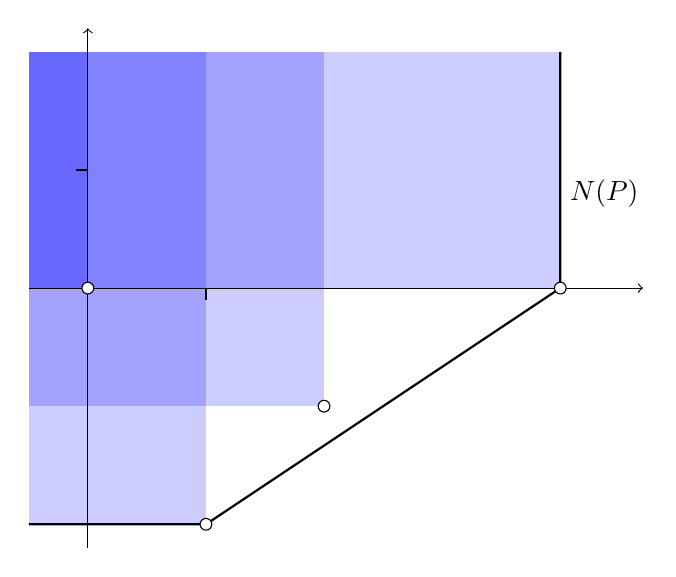
\begin{tikzpicture}[scale=1.5]
\def\myPoints{{(0,0)}, {(1,-2)}, {(2,-1)}, {(4,0)}}
\def\myPath{(-.5,-2) -- (1,-2) -- (4,0) -- (4,2)}
\myNewtonPlot{\myPoints}{\myPath}{4}{-2}{2}{$N(P)$}
\end{tikzpicture}
\end{lstlisting}
ergibt dann
\begin{center}
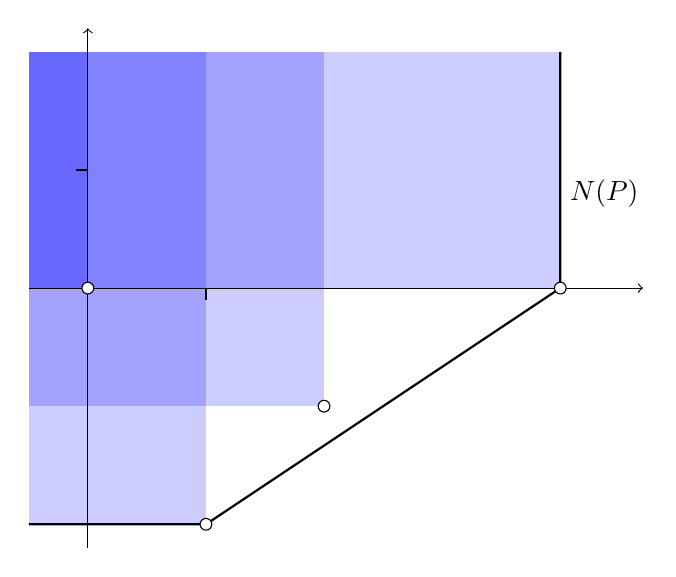
\begin{tikzpicture}[scale=1.5]
\def\myPoints{{(0,0)}, {(1,-2)}, {(2,-1)}, {(4,0)}}
\def\myPath{(-.5,-2) -- (1,-2) -- (4,0) -- (4,2)}
\myNewtonPlot{\myPoints}{\myPath}{4}{-2}{2}{$N(P)$}
\end{tikzpicture}
\end{center}

\newpage
BEGIN

\begin{center}
\begin{python}
print r"Hello \LaTeX!"
\end{python}
\begin{tikzpicture}[scale=1.5]
\def\myPoints{{{(0,0)}, {(1,1)}, {(2,1)}}}
\def\myXArr{0,1,2,3}
\def\myYArr{{0,1,1,4}}
\def\maxY{4}
\def\minY{0}

%rectangle
\foreach \x [count=\xi] in \myXArr {
  \pgfmathparse{\myYArr[\xi-1]}
  \def\y{\pgfmathresult}

  \fill[blue,opacity=.2] (-.5,\maxY+.5) rectangle (\x,\y);
}

%path
\foreach \x [count=\xi] in \myXArr {
  \pgfmathparse{\myYArr[\xi-1]}
  \def\y{\pgfmathresult}
  
  
}

%nodes
\foreach \x [count=\xi] in \myXArr {
  \pgfmathparse{\myYArr[\xi-1]}
  \def\y{\pgfmathresult}

  \node[draw,circle,inner sep=1.5pt,fill=white] at (\x,\y) {};
}
\end{tikzpicture}
\end{center}

END


% vim: set ft=tex :
